\chapter{SOLID}
SOLID ist ein Akronym, das fünf grundlegende Prinzipien des objektorientierten Designs zusammenfasst. Diese Prinzipien dienen dazu, die Struktur und Flexibilität von Software zu verbessern und die Codequalität zu erhöhen.
\begin{enumerate}
    \item Single Responsibility Principle (\textbf{SRP}): Eine Klasse sollte nur eine einzige Verantwortlichkeit haben und für eine spezifische Aufgabe zuständig sein.

    \item Open-Closed Principle (\textbf{OCP}): Klassen sollten offen für Erweiterungen, aber geschlossen für Modifikationen sein, indem sie neue Funktionen hinzufügen, ohne den bestehenden Code zu ändern.
    
    \item Liskov Substitution Principle (\textbf{LSP}): Subtypen sollten sich genauso verhalten wie ihre Basistypen, um eine nahtlose Austauschbarkeit zu gewährleisten.
    
    \item Interface Segregation Principle (\textbf{ISP}): Schnittstellen sollten spezifisch auf die Bedürfnisse der Clients zugeschnitten sein, sodass sie nur von den Methoden abhängig sind, die sie tatsächlich benötigen.
    
    \item Dependency Inversion Principle (\textbf{DIP}): Abhängigkeiten sollten auf abstrakte Konzepte oder Schnittstellen, nicht auf konkrete Implementierungen, ausgerichtet sein, um die Flexibilität und Austauschbarkeit von Komponenten zu fördern.
\end{enumerate}
\section{Analyse Single-Responsibility-Principle (SRP)}
Das Single Responsibility Principle (SRP) besagt, dass eine Klasse nur eine einzige Verantwortlichkeit haben sollte. Sie sollte für eine spezifische Aufgabe oder Funktion zuständig sein. Dadurch wird sichergestellt, dass die Klasse nur für einen bestimmten Aspekt der Funktionalität verantwortlich ist und sich nicht mit mehreren unterschiedlichen Aufgaben befasst. Das SRP ermöglicht eine bessere Lesbarkeit, Wartbarkeit und Testbarkeit des Codes, da jeder Verantwortungsbereich in einer separaten Klasse organisiert ist. Durch die Einhaltung des SRP können Änderungen oder Erweiterungen in einem Bereich vorgenommen werden, ohne dass andere Bereiche der Klasse betroffen sind.
\subsection{Positiv Beispiel}
\begin{figure}[ht]
    \centering
    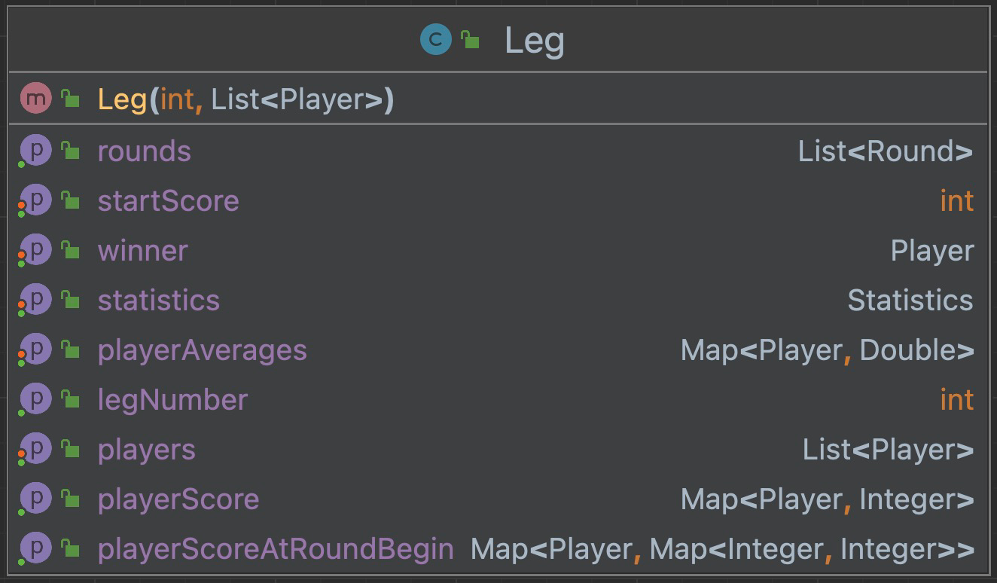
\includegraphics[width=0.8\textwidth]{Bilder/Leg.png}
    \caption{Leg Klasse}
    \label{fig:leg-uml}
\end{figure}
Diese Klasse hält das SRP ein, da sie nur die Aufgabe hat, Informationen über ein Leg eines Dart Spiels zu speichern. Zur Initialisierung des Legs werden 2 Informationen benötigt. Die Spieler, welche am Leg teilnehmen und die Anzahl der zu erreichenden Punkte. Während der Initialisierung wird das Attribut \textit{playerscore} deklariert und mit einer \textit{Map} initialisiert. Die \textit{Map} ermöglicht eine Zuordnung zwischen den Spielern und ihren Scores. Im \textit{statistics}-Objekt werden die Statistiken (Averages und checkout Quote)pro Spieler gespeichert. Zuvor war es nur möglich averages (im \textit{playerAverages}-Objekt) zu speichern. Dieses Attribut kann in den nächsten Updates der Applikation gelöscht werden. Die \textit{legNumber} speichert die Nummer des Legs, welche beispielsweise für die Ausgabe in der Konsole (\textit{Leg Nummer 3 wird nun gespielt...}) verwendet. \textit{playerScoreAtRoundBegin} speichert den Score des Spielers zu Beginn einer Runde. Dieses Attribut wird benötigt, um die Checkout Quote zu berechnen. Das \textit{rounds}-Attribut speichert die verschiedenen Runden des Legs und das \textit{winner}-Attribut speichert den Gewinner eines Legs.
\subsection{Negativ Beispiel}
\begin{figure}[ht]
    \centering
    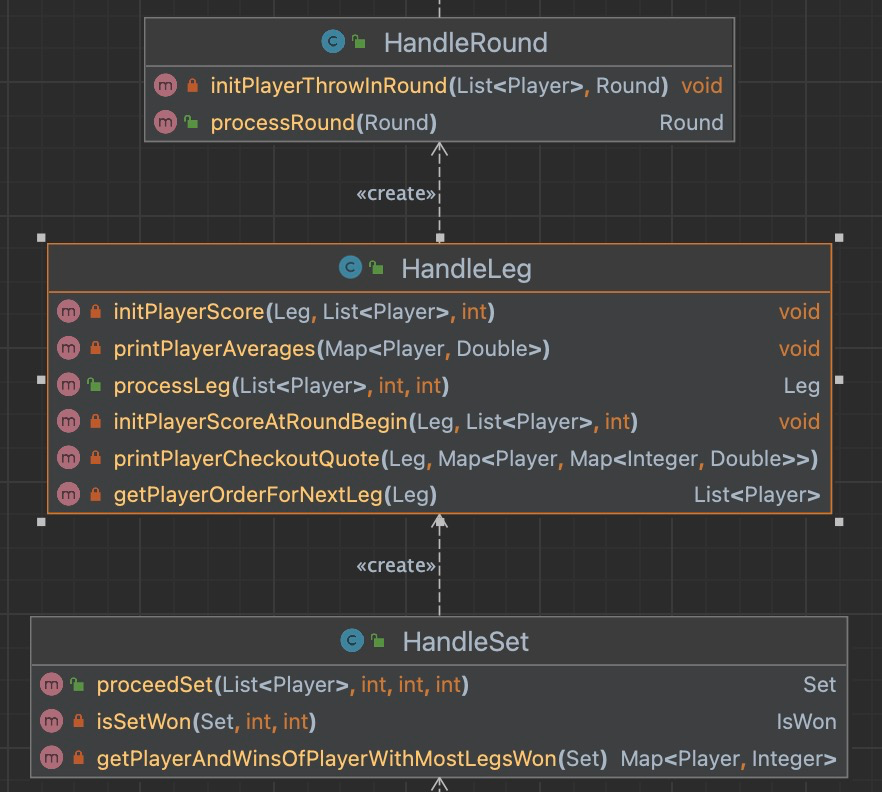
\includegraphics[width=0.8\textwidth]{Bilder/HandleLeg.png}
    \caption{HandleLeg Klasse}
    \label{fig:handleLeg-uml}
\end{figure}
Die HandleLeg-Klasse hält das SRP nicht vollständig ein, da sie eigentlich nur Logik für das Abarbeiten eines Legs beinhalten sollte. Die Logik des Legs befindet sich, wie auch bei den anderen Handle-Klassen, in der HandleLeg-Klasse, welche ein Leg-Objekt zurückgibt. Die Existenz der init-Methoden in der Klasse könnte auch schon als Argument genommen werden, um zu begründen, dass die Klasse das SRP nicht einhält, da diese Methoden auch in eine Klasse \textit{Setup} oder \textit{Init} ausgelagert werden könnten. Die beiden \textit{print}-Methoden verletzen das SRP jedoch deutlicher, da diese wenig mit dem Abarbeiten des Leg-Prozesses zu tun haben und ausgelagert werden können.
\section{Open Closed Principle (OCP)}

\subsection{Positiv Beispiel}
In der Leg-Klasse wird ein Statistics-Objekt verwendet, um verschiedene statistische Metriken zu speichern. Dies beinhaltet sowohl Durchschnittswerte, gespeichert in der \textit{averages}-Map, als auch Checkout-Informationen, die in der \textit{checkout}-Map gespeichert sind. Der Einsatz dieses Statistics-Objekts fördert die Einhaltung des Open-Closed-Prinzips (OCP).\\

Da das Statistics-Objekt für die Speicherung aller statistischen Werte verantwortlich ist, können neue Statistiken hinzugefügt oder vorhandene geändert werden, ohne die Leg-Klasse selbst zu modifizieren.\\

Sollte also eine Erweiterung um zusätzliche Statistiken erforderlich sein, würde dies lediglich eine Anpassung oder Erweiterung des Statistics-Objekts bedeuten. Die Leg-Klasse bleibt dadurch unverändert, wodurch das Risiko von Fehlern oder unerwarteten Seiteneffekten in diesem Teil des Systems minimiert wird. Dies unterstreicht, wie das Statistics-Objekt dazu beiträgt, das Open-Closed-Prinzip in der Anwendung einzuhalten.
\subsection{Negativ Beispiel}
Als negativ Beispiel können die verschiedenen Handle-Klassen betrachtet werden. Wenn beispielsweise ein weiterer Spielmodus hinzugefügt werden soll, muss jede Handle-Klasse angepasst werden. Beispielsweise ist das Kriterium für einen Checkout ein anderer bei bspw. Around the Clock als beim klassischen 501. Zum tracken der Punkte reicht auch keine normale Map mehr, sondern es wird eine separate Datenstruktur benötigt. Alle diese Änderungen würden dazu führen, dass die Handle-Klassen verändert werden müssten. Dies verstösst gegen das \acf{OCP}.
\section{\acf{ISP}}
\subsection{Positiv Beispiel}
\textbf{\acf{ISP}}\\
\begin{defStrich}[\acf{ISP}]
    Das \acf{ISP} ist ein Prinzip in der objektorientierten Programmierung, das besagt, dass keine Klasse aufgrund ihrer Schnittstellen von Methoden abhängig sein sollte, die sie nicht verwendet. Es gehört zu den fünf Prinzipien des SOLID-Ansatzes für das Software-Design. Mit anderen Worten, es ist besser, viele spezifische Schnittstellen zu haben als eine allgemeine; dies verhindert, dass eine Änderung in einer nicht verwendeten Methode einer Klasse zu einem unerwünschten Seiteneffekt in einer anderen Klasse führt. Das ISP hilft, den Code wartbarer und einfacher zu verstehen zu machen, indem es verhindert, dass Klassen mit ungenutzten Methoden überladen werden. Kurz gesagt, es fördert die Entkopplung von Software-Modulen und verbessert deren Flexibilität und Wiederverwendbarkeit.
\end{defStrich}
\begin{figure}[ht]
    \centering
    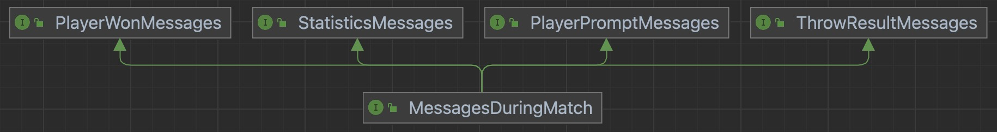
\includegraphics[width=0.8\textwidth]{Bilder/messagesDuringMatchUML.png}
    \caption{MessagesDuringMatch Interface UML}
    \label{fig:messagesDuringMatch-uml}
\end{figure}
Das Interface MessagesDuringMatch ist nicht monolithisch gestaltet, sondern in mehrere kleinere Interfaces unterteilt, die jeweils unterschiedliche Nachrichten während des Spielverlaufs repräsentieren. Diese Struktur entspricht dem Prinzip der \acf{ISP}. Im Falle, dass eine Klasse nur einen bestimmten Nachrichtentyp, wie zum Beispiel Statistikausgaben, benötigt, ermöglicht diese Struktur die Implementierung lediglich des relevanten Interfaces. Auf diese Weise wird eine effiziente und zielgerichtete Architektur erreicht.\newpage

\subsection{Negativ Beispiel}
\begin{figure}[ht]
    \centering
    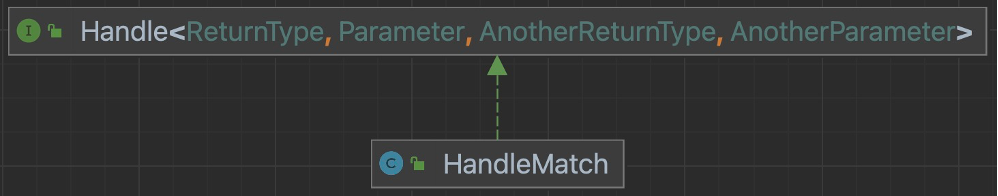
\includegraphics[width=0.8\textwidth]{Bilder/HandleInterfaceUML.png}
    \caption{Handle Interface UML}
    \label{fig:handleinterface-uml}
\end{figure}
Das Handle-Interface verstößt gegen das \ac{ISP}, da es Methoden enthält, die nicht von allen Implementierungen benötigt werden. Konkret werden zwei Methoden bereitgestellt, wobei die erste Methode in allen Implementierungen genutzt wird, die zweite jedoch lediglich in zwei von sechs Implementierungen. Dies führt zu einer unnötigen Abhängigkeit für die vier Implementierungen, die die zweite Methode nicht benötigen. Eine Lösung dieses Problems könnte in der Aufteilung des Handle-Interfaces in zwei separate Interfaces bestehen, wobei jedes Interface genau eine der beiden Methoden enthält. Alternativ könnte das Interface auch vollständig aufgelöst und durch andere Mechanismen ersetzt werden, um den Anforderungen des \ac{ISP} gerecht zu werden.
